%!TEX root = article.tex
\section{Experiments}\label{sec:exps}

We have introduced and stated convergence results on the online Sinkhorn
algorithm. These convergence results are non-quantitative and therefore require
an extensive experiment validation. Our experiments are three-fold: first, we
show that online Sinkhorn correctly estimates the solutions of
\eqref{eq:wass} and the Sinkhorn distance, overcoming the bias due to the fixed
a priori sampling of the regular Sinkhorn algorithm. Then, we show how online
Sinkhorn accelerates the Sinkhorn algorithm, by progressively estimating
sketches of the dual potentials, in parallel to the computation of the distance
matrix. Finally, we show how online Sinkhorn allows one to estimate accurately
the geometry of the dual, significantly improving the result using SGD with RKHS
expansions~\citep{2016-genevay-nips}. Numpy and Pytorch code are provided for experiment reproduction\footnote{\url{github.com/arthurmensch/online_sinkhorn}}.

\subsection{Better estimation of Sinkhorn distances}\label{sec:exp1}

\begin{figure}[t]
    \centering
    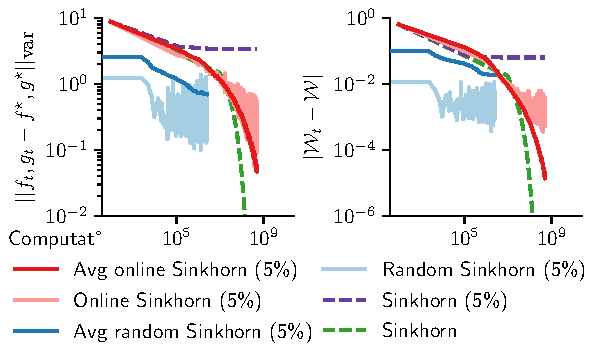
\includegraphics[width=\linewidth]{comparison.pdf}

    \vspace{-1em}

    \caption{Comparison of online, random and fixed sampling Sinkhorn performances. Online Sinkhorn overcomes the bias of sampling---especially with out-of-loop averaging. Random Sinkhorn gives fast estimations, whose variance does not decrease.}
    \label{fig:convergence}
\end{figure}


We first consider a discrete distribution $(\alpha, \beta)$, to be able to
compute the reference distance $\Ww = \Ww(\alpha, \beta)$ and the optimal
potentials $f^\star$, $g^\star$, using Sinkhorn algorithm. The goal here is not
to perform better than the Sinkhorn algorithm in the long run. Indeed, the
constraints of online Sinkhorn impose unnecessary slow-downs when dealing with
small discrete distributions. Rather, our purpose is to illustrate the improved
precision of online Sinkhorn for estimating true OT distances. We choose $\alpha$ and $\beta$ to be two
discrete 1-D distributions, $\Xx=\RR$, sampled from the continuous densities
displayed in
\autoref{fig:potentials}. We set $\varepsilon = 10^{-2} \max_{x,y}
C(x,y)$, where we use the squared Euclidean loss (regularized $\Ww_2$
setting)---the distributions $\alpha$ and $\beta$ have bounded support. We use
$\eta_t = \frac{1}{\sqrt{t}}$ for online Sinkhorn and a fixed batch-size $n$, in
all experiments. We compare the performance of Sinkhorn, online Sinkhorn and
random Sinkhorn, measuring $\Vert f - f^\star \Vert_{\text{var}} + \Vert g -
g^\star \Vert_{\text{var}}$ and the absolute error $| \Ww_t - \Ww |$ versus the
number of computations performed---the evaluation of $C(x_i, y_i)$ and the
computation of each addition in the $C$-transform being considered as elementary
computation units. We further report the performance of using out-of-loop
averaging with $\gamma_t = \frac{1}{\sqrt{t}}$.

\paragraph{Results.} We report convergence curves in \autoref{fig:convergence}.
Compared to the subsampled Sinkhorn algorithm that computes a biased estimate of
the distance $\Ww$ (purple), the online Sinkhorn algorithm successfully
estimates the distance and the associated potentials, despite performing only
partial $C$-transforms (red). Random Sinkhorn (blue) finds a decent estimation
of the distance and potentials, with fewer computations than the full Sinkhorn
algorithm, but fails to converge. Averaging the random Sinkhorn iterations finds
a biased estimation. The vanilla online Sinkhorn yields values that are much
closer to the true OT distance, albeit with a rather high iterate variance (note
that this variance does reduce---this is a log-log plot). Remarkably, the
out-of-loop averaging of online Sinkhorn enjoys much better converging
property---we confirmed this finding on many synthetic problems. It is
surprising that an averaging mechanism brings speed-up in a non-convex
setting---we attribute this to the convexity of the original problem, although
this should be further investigated.

\begin{figure}[t]
    \centering
    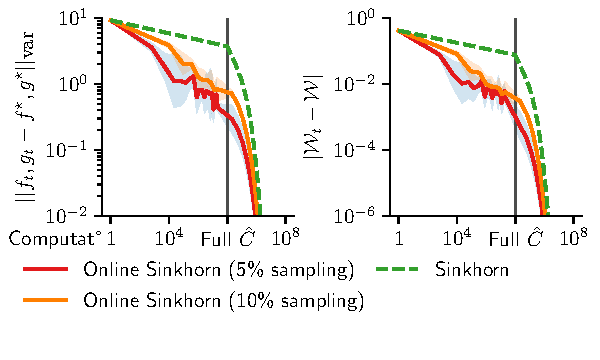
\includegraphics[width=\linewidth]{early_compute}
    
    \vspace{-1em}

    \caption{Using online Sinkhorn during the initial computation of the cost
     matrix accelerates the Sinkhorn algorithm: it provides good estimates of
     the potentials $f$ and $g$ to warm start the full Sinkhorn algorithm.
     Curves averaged over 5 runs. \label{fig:early_compute}}
\end{figure}

\begin{figure*}[t]
    \centering
    \if\icml0
    \begin{widepage}
    \fi
    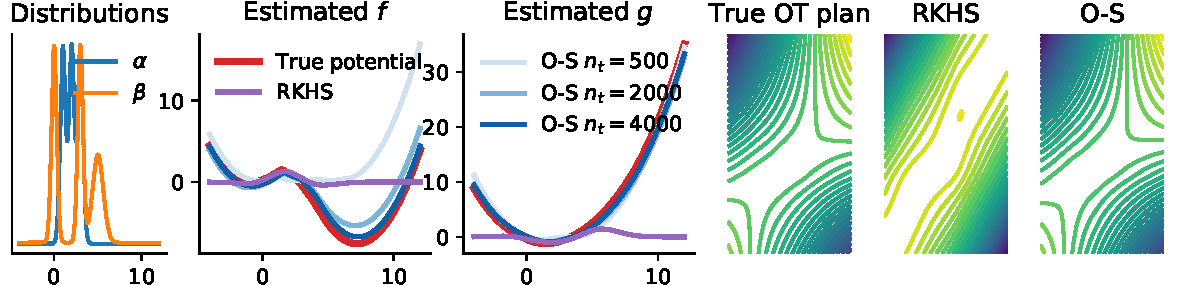
\includegraphics[width=\linewidth]{continuous.pdf}
    \caption{Representation of the convergence path of online Sinkhorn: the blue curves represents the estimated potentials (continuous functions) at different stages of the algorithm. The estimated plan $\pi_t$ is very quickly accurate, while the shape of the potentials match nearly perfectly the true potentials (estimated on a grid $N = 5000$). $\varepsilon = 10^{-2} \max \hat C$.
    \label{fig:potentials}
    }
    \if\icml0
    \end{widepage}
    \fi
\end{figure*}

\subsection{Accelerating the first Sinkhorn iteration}\label{sec:accelerating}

The discrete Sinkhorn algorithm requires to compute the full cost matrix $\hat C \eqdef
(C(x_i,y_i))_{i,j}$  of size $N \times N$, prior to estimating the
potentials $f_1$ and $g_1$ by a first $C$-transform. In contrast, online Sinkhorn can progressively
computes this matrix while computing first sketches of the potentials. We therefore
assess the performance of the following \textit{online+full Sinkhorn} algorithm
in a discrete setting: online Sinkhorn is run with batch-size $n$ during the first iterations, until
observing each sample of $[1,N]$, i.e. until the cost matrix $C$ is completely evaluated. The discrete instantion of online Sinkhorn is derived in \autoref{sec:sinkhorn_discrete}, \autoref{alg:discrete_online}. 
At this point (iteration $t$), online Sinkhorn provides the estimates $f_{t},
g_{t}$. From then, the algorithm only performs full Sinkhorn updates.


\paragraph{Results.} We report convergence curves in
\autoref{fig:early_compute}. The proposed scheme indeed provides an improvement
upon Sinkhorn algorithm. After $N^2$ computation (the cost of estimating the
full matrix $\hat C$), both the function value and distance to optimum are lower
using our scheme: the full Sinkhorn algorithm then operates from a good
initialization for potentials. Computing those cost approximately as much as
estimating the matrix $\hat C$ in dimension $1$. The \textit{online+full}
Sinkhorn algorithm then maintains an advantage over the full Sinkhorn algorithm
over time. Note that the cost of estimating initial potentials becomes negligible
as the dimension increase---the cost of computing $\hat C$ dominates. This
strongly advocates for using an online scheme as a warm-up for regularized OT
estimation. We note that using smaller batch-size $n$ may lead to higher speed-up (here, $n=50$ performs better than $n=100$).
There is an optimal $n$. The speed gain decreases with $\epsilon$, but remains
significant even for $\epsilon = 10^{-4} \max \hat C$. We add that
using a sampling-without-replacement scheme brings an additional speed-up. Out-of-loop averaging is also beneficial. We refer to \autoref{sec:supp_exp} for an additional experiment with a lower $\varepsilon$.

\subsection{Continuous potential estimation}

Finally, we measure the performance of our algorithm in a truly continuous
setting, where $\alpha$ and $\beta$ are $1$-D parametric distributions (Gaussian
mixtures) from which we sample. In the absence of reference $\Ww$ (which cannot be accurately computed
without a method akin to ours), we monitor the
trajectories of the potentials, and compare them to the Sinkhorn potentials for
realization of $\alpha$ and $\beta$ of size $n=2000$. We also monitor the
estimated transportation plan $\hat \pi_t = (\alpha \otimes \beta)
\exp(\frac{f\oplus g - C}{\varepsilon}) \in \Mm^+(\Xx)^2$. We run the experiments with
$n_T=5000$.

\paragraph{Results.} We show the convergence trajectories of the potentials in
\autoref{fig:potentials}. Online Sinkhorn refines the potentials $(f_t, g_t)_t$ until convergence. The fact that our method uses an adapted potential parametrization~\eqref{eq:param}
allows the iterates to quickly identify the correct shape of the optimum. The
final plan is undistinguishable from the true transportation plan. Quantitative
values (distance to true potentials, error in Sinkhorn distance estimation) converge as in
\autoref{fig:convergence}.

\paragraph{Comparison to concurrent approaches.}\label{sec:compare}Finally, we compare the online
Sinkhorn algorithm to constructing representations of Sinkhorn potentials using universal
RKHS \citep{2016-genevay-nips}. This competing approach sets $f_t(\cdot) =
\sum_{i=1}^{n_t} \alpha_t \kappa(\cdot, x_i)$ (and similarly for $g_t$), where $\kappa$ is
a reproducing kernel (typically a Gaussian). This differs significantly from the
representations that we propose, for which $\exp(-f_t)$, and not $f_t$, is
expressed as a kernel mixture. 
%
With RKHS representations of potentials, the
dual problem \eqref{eq:sinkhorn} can be solved using stochastic gradient
descent, with theoretical convergence guarantees. As advocated by the authors,
we run a grid search over the bandwidth parameter~$\sigma$ of the Gaussian kernel to select the best
performing runs. We set $n_T = 50000$, and $\epsilon = 10^{-1} \max C$. We could not successfully use the RKHS method for lower $\epsilon$.

We compare the final potentials and associated transportation plans in
\autoref{fig:comparison_rkhs}. Our method estimates potentials with much less
errors, especially in areas where the mass of $\alpha$ and $\beta$ is low. The
computational complexity of both algorithms are comparable. Online Sinkhorn does
not require to set any hyperparameters, whereas we observed that SGD in RKHS is very
sensitive to bandwidth selection.

\begin{figure}[t]
    \centering
    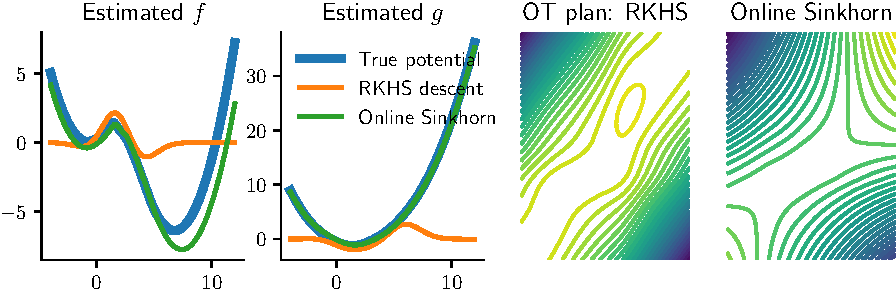
\includegraphics[width=\linewidth]{continuous_francis-crop.pdf}
    \caption{Comparing online Sinkhorn with SGD over a RKHS representation of the potential \citep{2016-genevay-nips}, with best bandwidth parameter. Online Sinkhorn finds more accurate functional representations of potentials, thanks to its more appropriate parametrization. $\varepsilon = 10^{-1} \max \hat C$.}
    \label{fig:comparison_rkhs}
\end{figure}